\documentclass[../lab2.tex]{subfiles}

\begin{document}
\begin{figure}[!htb]
    \begin{minipage}{0.48\textwidth}
        \centering
        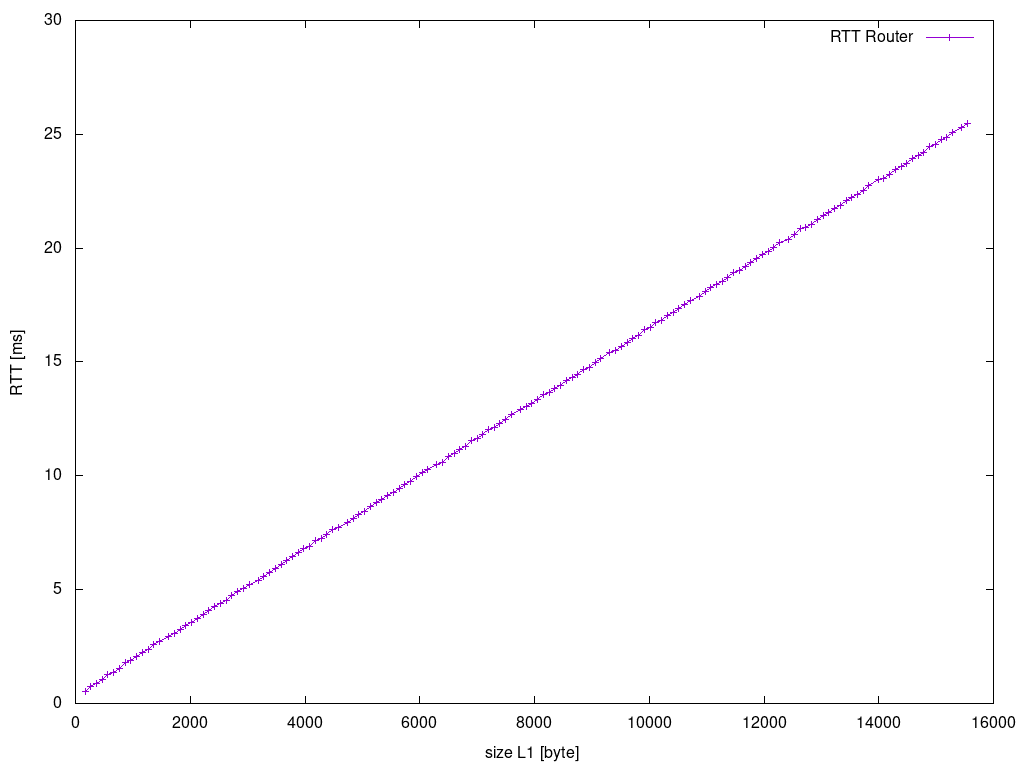
\includegraphics[width=1\linewidth]{RTTR.png}
        \vspace{-20pt}
        \caption{RTT}\label{RTTR}
    \end{minipage}\hfill
    \begin{minipage}{0.48\textwidth}
        \centering
        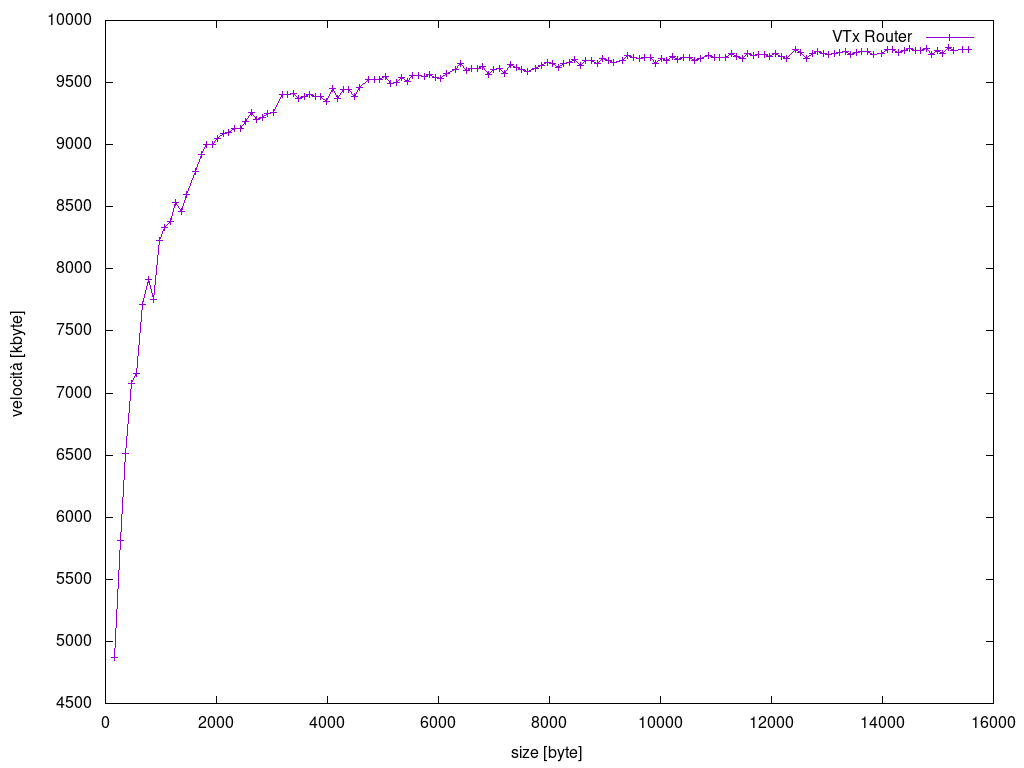
\includegraphics[width=1\linewidth]{VTxR.png}
        \vspace{-20pt}
        \caption{VTx}\label{VTxR}
    \end{minipage}
\end{figure}

In questo caso si rielaborano le formule (2) (4) nel modo seguente:

\begin{equation}
    \centering
    RTT = 2T_{TX} + T_{\eta}
\end{equation}

\begin{equation}
    \centering
    V_{TX} = \frac{2D(s)}{RTT}
\end{equation}

Coinvolgendo solamente due dispositivi collegati mediante un cavo ethernet di modesta lunghezza
il comportamtno riscontrato è soggetto a meno variazioni ed è molto simile al comportamento 
teorizzato.

\end{document}